\subsection{Black Hole Evaporation and the Information Problem}
  \label{subsec:black-hole-evaporation-information}

  Within the Cosmochrony framework, black holes are not associated with physical
  singularities, but with regions where spacetime projection ceases to be injective.
  Such regions define domains of limited representability rather than physical interiors.

  \paragraph{Evaporation as a Projective Phenomenon.}
    Black hole evaporation is an effective process unfolding entirely within the
    projectable regime.
    It arises from the gradual restoration of projectability near the boundary separating
    projectable and non-projectable domains.

    As projectability is progressively recovered, localized projected configurations
    cease to be supported and are replaced by radiation-like effective descriptions.
    The evaporation process completes before any effective description would encounter a
    non-projectable singular regime.

  \paragraph{Resolution of the Information Paradox.}
    The apparent information loss identified by Hawking arises from treating spacetime as
    fundamental~\cite{Hawking1976}.
    In Cosmochrony, information is encoded in the global relational configuration
    independently of its spacetime projection.
    Evaporation therefore does not violate unitarity; it reflects a change in the domain
    of representability.

  \paragraph{Observational Implications.}
    To external observers, emitted radiation appears nearly thermal and weakly
    correlated with infalling states.
    This reflects the coarse-grained nature of spacetime projection rather than genuine
    information loss.
    The black hole information paradox is thus resolved by recognizing it as an artifact
    of extrapolating spacetime concepts beyond their domain of validity.

\subsubsection*{Horizon Reprojection Equation}
  \label{subsec:horizon-reprojection-equation}

  Within Cosmochrony, black hole evaporation is described as a reprojection process
  by which structural energy stored in the $\chi$ substrate is released into the projected
  spacetime in discrete units.

  The energy flux emerging from the horizon is defined as a sum over reprojection
  events associated with micro-configurations of the projection fiber:
  \[
    \Phi_\chi \equiv \frac{dE}{dt}
    = \sum_k \delta(t - t_k)\, \hbar_\chi\, \nu_k(L_{\mathrm{sol}}).
  \]

  Here, $\hbar_\chi$ denotes the fundamental quantum of reprojection, setting the
  minimal granularity of projected action.
  The quantities $\nu_k(L_{\mathrm{sol}})$ correspond to the resonance frequencies
  associated with the eigenmodes of the stability operator $L_{\mathrm{sol}}$ acting
  on the projection fiber $\Pi^{-1}(g_H)$ at the horizon, where $g_H$ denotes the
  effective near-horizon geometry.
  The times $t_k$ label the instants at which local $\chi$ configurations reach the
  projection threshold and become effectively visible in spacetime.

  Black hole evaporation thus proceeds as a sequence of discrete reprojection pulses,
  rather than as a continuous emission process.

\subsubsection*{Emergent Temperature and Relaxation Gradient}
  \label{subsec:emergent-temperature}

  The apparent Hawking temperature perceived by a distant observer emerges from the
  statistical distribution of reprojection events.
  It is determined by the gradient of effective $\chi$ relaxation normal to the horizon.

  This relation may be expressed as
  \[
    k_B T_\chi = \frac{\hbar_\chi c}{2\pi}\,
    \left| \nabla_{\perp} \chi_{\mathrm{eff}} \right|_H.
  \]

  For more massive black holes, the relaxation gradient is distributed over a larger
  horizon area, reducing the frequency of reprojection events.
  This directly explains the inverse mass–temperature relation without invoking
  vacuum particle creation or fundamental thermodynamic assumptions.

\subsubsection*{Information Conservation and Spectral Encoding}
  \label{subsec:information-conservation}

  In contrast with semiclassical descriptions, information is never destroyed in
  Cosmochrony.
  The projection operator $\Pi$ acts as a filter rather than as an irreversible map.

  During the deprojection phase, information is stored in the nonlinear degrees of
  freedom of the $\chi$ substrate, encoded within the projection fiber.
  During reprojection, the emitted radiation carries the precise spectral imprint of
  the eigenmodes governing the $\chi$ configuration.

  Each emitted quantum corresponds to a specific transition within the substrate,
  ensuring global unitarity.
  The apparent loss of information arises solely from restricting attention to the
  projected metric degrees of freedom.

\subsubsection*{Entropy as a Projection Saturation Limit}
  \label{subsubsec:entropy-projection-saturation}

  Within the Cosmochrony framework, the recovery of the Bekenstein--Hawking
  area law,
  \begin{equation}
    S = \frac{A}{4},
  \end{equation}
  does not rely on the introduction of a temperature or on thermodynamic
  postulates.
  Instead, black hole entropy is reinterpreted as a measure of the
  informational capacity of the projection map $\Pi$ at the horizon boundary.

  \paragraph{The Horizon as a De-projection Boundary}

    In the near-horizon regime, the $\chi$ substrate approaches a state of
    critical constraint in which the mapping
    \(
    \Pi : \chi \rightarrow g_{\mu\nu}
    \)
    ceases to be injective (see Section~7.7.3).
    The horizon is therefore redefined as the locus at which the local
    relaxation rate $N(r)$ vanishes, preventing further refinement of the
    projected metric degrees of freedom.

    At this boundary, distinct micro-configurations of the substrate are
    mapped onto the same effective horizon geometry $g_H$.
    Entropy is identified with the logarithmic measure of the fiber
    \(
    \Pi^{-1}(g_H),
    \)
    that is, the structural multiplicity of $\chi$ configurations that are no
    longer distinguishable at the metric level.
    Entropy thus quantifies hidden relational structure, rather than thermal
    ignorance.

    This situation is schematically illustrated in
    Figure~\ref{fig:projection-saturation-horizon}.

    \begin{figure}[htbp]
      \centering
      \resizebox{\linewidth}{!}{%
        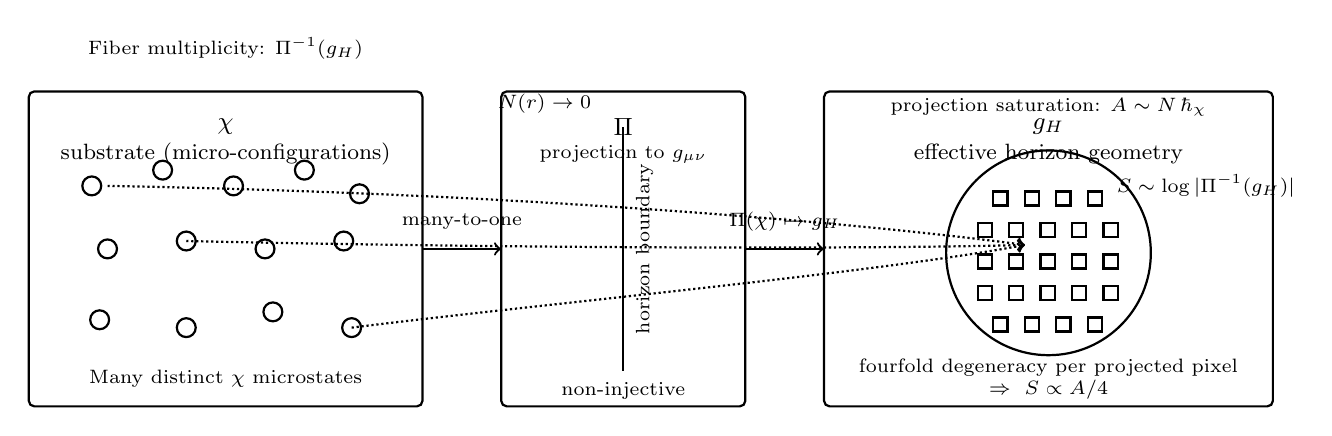
\begin{tikzpicture}[font=\small]

          % --- Geometry constants (implicit): boxes are placed in absolute coordinates ---
          % Left box: chi
          \draw[thick,rounded corners=2pt] (0,0) rectangle (5.0,4.0);
          \node at (2.5,3.55) {$\chi$};
          \node[font=\footnotesize] at (2.5,3.20) {substrate (micro-configurations)};

          % Middle box: projection / horizon boundary
          \draw[thick,rounded corners=2pt] (6.0,0) rectangle (9.1,4.0);
          \node at (7.55,3.55) {$\Pi$};
          \node[font=\scriptsize] at (7.55,3.20) {projection to $g_{\mu\nu}$};

          % Right box: g_H (keep minimal to avoid overlap)
          \draw[thick,rounded corners=2pt] (10.1,0) rectangle (15.8,4.0);
          \node at (12.95,3.55) {$g_H$};
          \node[font=\footnotesize] at (12.95,3.20) {effective horizon geometry};

          % --- Microstates (left box) ---
          \foreach \x/\y in {0.8/2.8,1.7/3.0,2.6/2.8,3.5/3.0,4.2/2.7,
          1.0/2.0,2.0/2.1,3.0/2.0,4.0/2.1,
          0.9/1.1,2.0/1.0,3.1/1.2,4.1/1.0}{
            \draw[thick] (\x,\y) circle (0.12);
          }
          \node[font=\scriptsize] at (2.5,0.35) {Many distinct $\chi$ microstates};

          % --- Arrow to middle box ---
          \draw[->,thick] (5.0,2.0) -- (6.0,2.0);
          \node[font=\scriptsize] at (5.5,2.35) {many-to-one};

          % --- Horizon boundary line inside middle box ---
          \draw[thick] (7.55,0.45) -- (7.55,3.55);
          \node[font=\scriptsize,rotate=90] at (7.82,2.0) {horizon boundary};
          \node[font=\scriptsize] at (6.55,3.85) {$N(r)\to 0$};
          \node[font=\scriptsize] at (7.55,0.20) {non-injective};

          % --- Arrow to right box ---
          \draw[->,thick] (9.1,2.0) -- (10.1,2.0);
          \node[font=\scriptsize] at (9.6,2.35) {$\Pi(\chi)\mapsto g_H$};

          % --- Horizon disk + pixels (right box) ---
          \draw[thick] (12.95,1.95) circle (1.30);
          \node[font=\scriptsize] at (12.95,3.80) {projection saturation: $A \sim N\,\hbar_\chi$};

          % pixels inside the disk (all are safely inside)
          \foreach \x/\y in {12.25/2.55,12.65/2.55,13.05/2.55,13.45/2.55,
          12.05/2.15,12.45/2.15,12.85/2.15,13.25/2.15,13.65/2.15,
          12.05/1.75,12.45/1.75,12.85/1.75,13.25/1.75,13.65/1.75,
          12.05/1.35,12.45/1.35,12.85/1.35,13.25/1.35,13.65/1.35,
          12.25/0.95,12.65/0.95,13.05/0.95,13.45/0.95}{
            \draw[thick] (\x,\y) rectangle ++(0.18,0.18);
          }

          % --- Dotted arrows: selected microstates collapse to same horizon pixel ---
          \draw[->,thick,densely dotted] (1.0,2.8) .. controls (6.5,2.7) and (10.8,2.3) .. (12.65,2.05);
          \draw[->,thick,densely dotted] (2.0,2.1) .. controls (6.5,2.0) and (10.8,2.0) .. (12.65,2.05);
          \draw[->,thick,densely dotted] (4.1,1.0) .. controls (6.5,1.3) and (10.8,1.7) .. (12.65,2.05);

          % --- External annotations (kept outside boxes to avoid overlap) ---
          \node[font=\scriptsize,align=left] at (2.5,4.55) {Fiber multiplicity: $\Pi^{-1}(g_H)$};
          \node[font=\scriptsize,align=left] at (14.95,2.80) {$S \sim \log |\Pi^{-1}(g_H)|$};
          \node[font=\scriptsize,align=center] at (12.95,0.35)
            {fourfold degeneracy per projected pixel\\$\Rightarrow\ S \propto A/4$};

        \end{tikzpicture}%
      } % resizebox

      \caption{
        Saturation of the projection map at the horizon.
        Near the boundary where $N(r)\to 0$, the projection $\Pi$ becomes non-injective:
        multiple micro-configurations of the $\chi$ substrate collapse onto the same
        effective horizon geometry $g_H$.
        Entropy measures the structural multiplicity of the fiber $\Pi^{-1}(g_H)$ and the
        saturation of projected metric ``pixels'' of area $\sim \hbar_\chi$.
      }
      \label{fig:projection-saturation-horizon}
    \end{figure}

  \paragraph{Geometric Origin of the \texorpdfstring{$1/4$}{1/4} Factor}

    The numerical factor $1/4$ arises as a structural ratio between the
    internal degrees of freedom of the $\chi$ substrate and their maximal
    holographic projection onto a two-dimensional boundary.

    Let $\hbar_\chi$ denote the elementary quantum of reprojection.
    The horizon area $A$ is saturated by a finite number $N$ of effective
    pixels of area $\sim \hbar_\chi$.
    Within the Cosmochrony framework, each such projected pixel corresponds to
    a fourfold degeneracy in the stability spectrum of $\chi$, linked to the
    intrinsic $4\pi$ periodicity of $\chi$ excitations discussed in
    Section~5.2.

    The area law
    \(
    S = A/4
    \)
    is therefore the macroscopic signature of this quadrature constraint:
    it represents the maximal density of independent structural degrees of
    freedom that can be projected before the non-injectivity of $\Pi$ induces
    a complete loss of local metric resolution.

  \paragraph{Unitary Reprojection and Information Conservation}

    Black hole evaporation is reformulated as a discrete reprojection
    process.
    As the $\chi$ substrate locally relaxes at the horizon boundary, it emits
    quanta of action $\hbar_\chi$ carrying the spectral imprint of the fiber
    $\Pi^{-1}(g_H)$.

    Because this process is governed by the deterministic---though
    nonlinear---relaxation dynamics of $\chi$, information is never destroyed
    nor trapped in a singularity.
    Instead, it is transferred from a purely structural encoding within the
    fiber back into observable spacetime degrees of freedom.
    Unitarity is preserved at the level of the $\chi$ substrate, even though
    the effective spacetime description may exhibit apparent non-unitarity.

  \paragraph*{Conclusion}

    In Cosmochrony, black hole entropy is not a measure of ignorance but a
    measure of projection saturation.
    It quantifies the threshold at which the complexity of the $\chi$
    substrate exceeds the transmittance capacity of the effective metric
    projection.
    This explains why entropy scales with area---the projection surface---and
    not with volume, which characterizes the inaccessible internal fiber.
